% Single-pass cross-referencing in LuaLaTeX: hold and patch.
% A TUGboat article about the monoref package.
\documentclass{ltugboat}

\usepackage{microtype}
\usepackage{graphicx}
\usepackage{xcolor}
\usepackage{listings}
\usepackage{tikz}
\usepackage{fontawesome5}
\usetikzlibrary{arrows.meta,positioning,shapes.geometric}

\definecolor{codeblue}{rgb}{0.05,0.22,0.48}
\definecolor{codegreen}{rgb}{0.00,0.38,0.18}
\definecolor{codered}{rgb}{0.55,0.12,0.10}
\definecolor{codegray}{gray}{0.35}
\definecolor{codeback}{gray}{0.97}

\lstdefinestyle{monorefcode}{%
  basicstyle=\ttfamily\small,
  keywordstyle=\bfseries\color{codeblue},
  commentstyle=\itshape\color{codegreen},
  stringstyle=\color{codered},
  identifierstyle=\color{black},
  backgroundcolor=\color{codeback},
  rulecolor=\color{black!25},
  frame=single,
  framerule=.25pt,
  framesep=2pt,
  columns=fullflexible,
  keepspaces=true,
  breaklines=true,
  breakatwhitespace=true,
  showstringspaces=false,
  aboveskip=.7\baselineskip,
  belowskip=.7\baselineskip,
}
\lstdefinestyle{monoreftex}{%
  style=monorefcode,
  language={[LaTeX]TeX},
  texcsstyle=*\bfseries\color{codeblue},
  moretexcs={AddToHook,DiscardShipoutBox,ShipoutBox,
    monorefslotwidth,monorefreftemplate,monorefpagetemplate,
    monoref@slot,monoref@tmpwd,monoref@slotattr,monoref@mark,
    monoref@markattr,monoref@tocline,monoref@indent,
    monoref@link,monoref@target,monoref@hyper,lastpage}
}
\lstdefinelanguage{MonorefLua}{%
  sensitive=true,
  morekeywords={local,function,then,elseif,end,for,do,return,and,or,if},
  morecomment=[l]{--},
  morestring=[b]",
  morestring=[b]',
}
\lstdefinestyle{monoreflua}{%
  style=monorefcode,
  language=MonorefLua,
  emph={monoref,node,tex,font,nil,true,false},
  emphstyle=\color{codeblue}
}

\title{Single-pass cross-referencing in \LuaLaTeX: hold and patch}
\shortTitle{Single-pass cross-referencing in \LuaLaTeX}
\author{Srikanth Mohankumar}
\address{TNQ Tech Pvt. Ltd.\\
Chennai, Tamilnadu, India}
\netaddress{srikanth.mohan@tnqtech.com}
\author{Nareshkumar Krishnaswamy}
\address{TNQ Tech Pvt. Ltd.\\
Chennai, Tamilnadu, India}
\netaddress{nareshkumar.k@tnqtech.com}

\begin{document}
\raggedbottom
\maketitle

\begin{abstract}
The \tbcode{monoref} package resolves a bounded set of \LaTeX{}
cross-references in one \LuaLaTeX{} run: \cs{ref}, \cs{pageref}, a
body-page total, and a generated table of contents.  It does this by
holding finished pages as Lua node lists, recording the true page of
labels with invisible markers, and replacing reserved reference slots
just before final shipout.  This article describes the implementation
and its trade-offs.
\end{abstract}

\section{The two-pass problem}

\LaTeX{} cross-references are normally a file-based fixed point.  On
one run, commands such as \cs{label} write label values and page
numbers to the \tbcode{.aux} file.\footnote{The \tbcode{.aux} file is
also used for many other document-level facts; \tbcode{monoref} only
addresses the reference subset described here.}  On the next run,
\cs{ref} and \cs{pageref} read those values back.  If the new values
differ from the old ones, another run may be needed.  Build tools such as
\tbcode{latexmk} automate that loop, but the document still depends on
state from a previous compilation.

The difficulty is especially clear for a forward reference:
\begin{lstlisting}[style=monoreftex]
\section{Intro}\label{sec:intro}
See Section~\ref{sec:res}.
...
\section{Results}\label{sec:res}
\end{lstlisting}
When the first paragraph is broken into lines, the value of
\tbcode{sec:res} has not yet been seen.  In standard \LaTeX{}, the
earlier run supplies the answer.  \tbcode{monoref} instead delays the
commit: it lets \TeX{} build pages, but it does not write them to the
\PDF{} file until the end of the document.

The scope is deliberately limited.  The package is not a general
replacement for the \tbcode{.aux} file.  It covers numbered labels,
page references, \cs{lastpage}, and a contents list for
\cs{section}, \cs{subsection}, and \cs{subsubsection}.  The constraint
makes a one-run implementation practical.

\begin{figure}
\centering
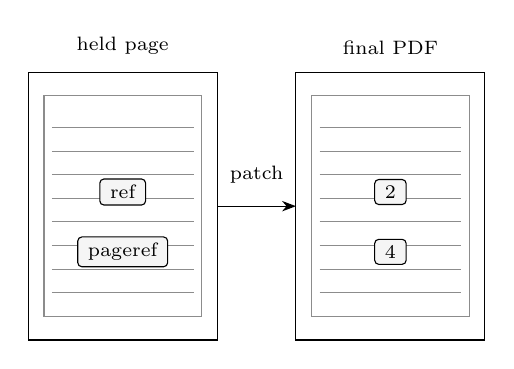
\begin{tikzpicture}[
  x=1mm,y=1mm,
  page/.style={draw, fill=white, minimum width=24mm, minimum height=34mm},
  line/.style={draw=black!45, line width=.35pt},
  note/.style={font=\scriptsize, align=center},
  tag/.style={draw, rounded corners=1.5pt, fill=black!4,
    inner xsep=1.3mm, inner ysep=.8mm, font=\scriptsize}
]
\node[page] (held) at (0,0) {};
\node[page] (final) at (34,0) {};
\node[note, above=1mm of held] {held page};
\node[note, above=1mm of final] {final PDF};
\foreach \y in {10,7,4,1,-2,-5,-8,-11}
  \draw[line] (-9,\y) -- (9,\y);
\foreach \y in {10,7,4,1,-2,-5,-8,-11}
  \draw[line] (25,\y) -- (43,\y);
\node[tag] at (0,1.8) {\cs{ref}};
\node[tag] at (0,-5.8) {\cs{pageref}};
\node[tag] at (34,1.8) {2};
\node[tag] at (34,-5.8) {4};
\draw[->, >=Stealth, line width=.45pt] (12,0) -- (22,0);
\node[note] at (17,4) {patch};
\draw[draw=black!45] (-10,-14) rectangle (10,14);
\draw[draw=black!45] (24,-14) rectangle (44,14);
\end{tikzpicture}
\caption{A reader sees ordinary references; internally the early page
contains attributed slots until finalization.}
\label{fig:mock-output}
\end{figure}

\section{Pipeline}

The implementation is a hold-and-patch pipeline.  Figure~\ref{fig:wide-comparison}
shows the order.  Pages produced by the page builder are copied into
Lua tables.\footnote{The page is kept as a Lua node list, not rendered to an
intermediate image or external file.}  As each page is held, a marker scan
assigns labels and TOC
entries to the page on which they actually appear.  After the input
stream ends, all slots are patched, lines containing slots are
repacked, the generated contents pages are added ahead of the body, and
the queued pages are shipped for real.

\begin{figure*}
\centering
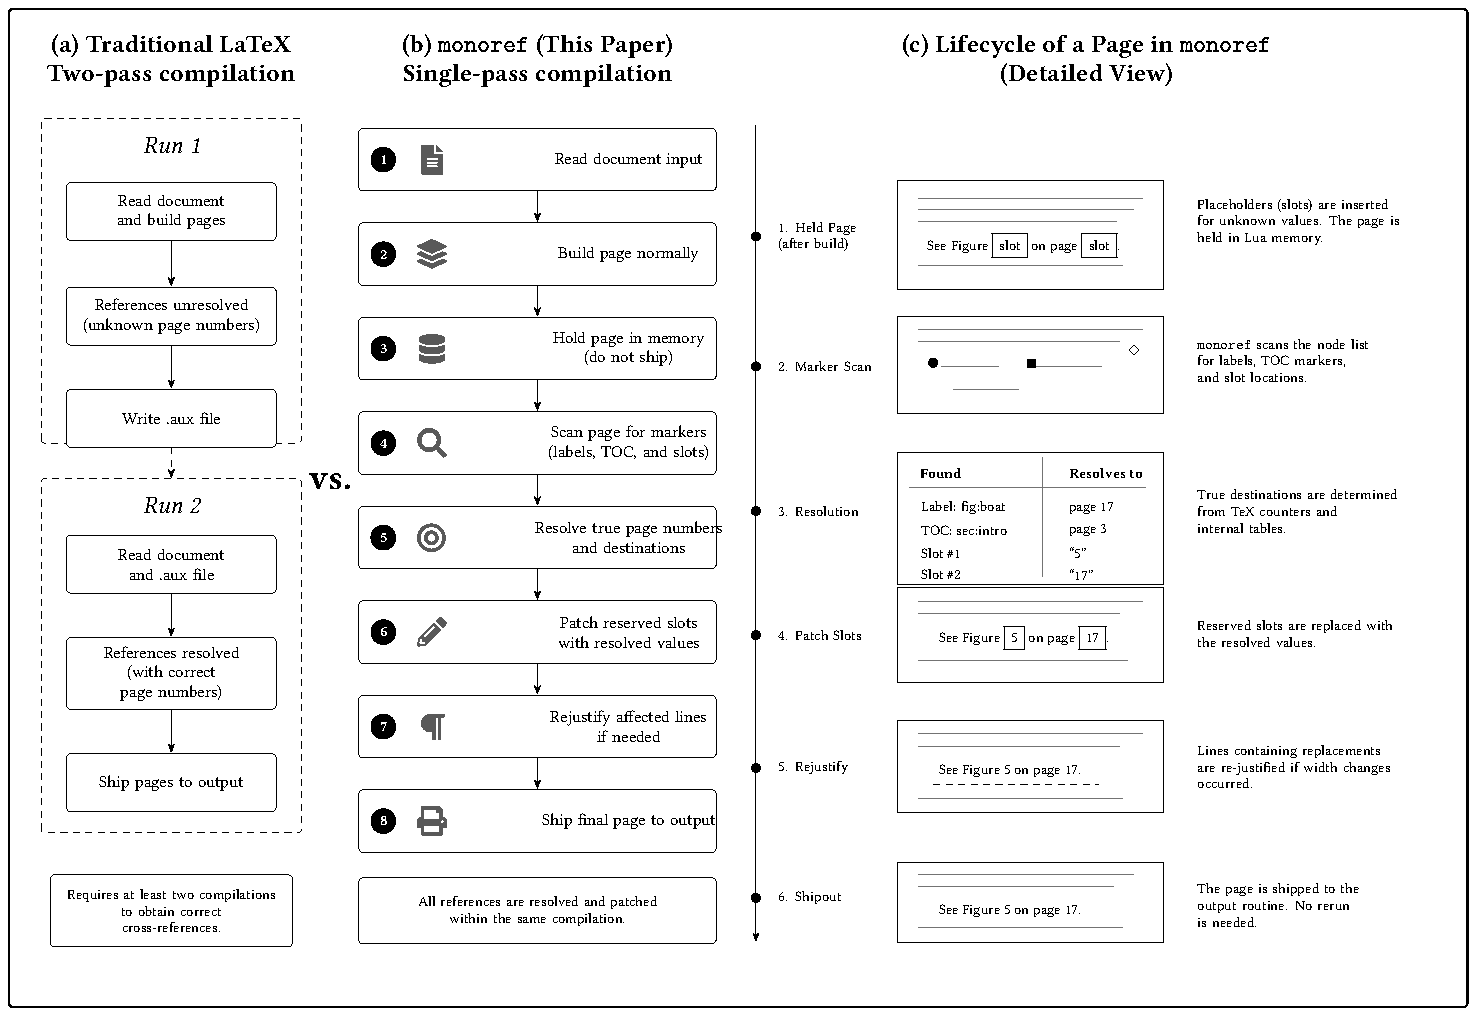
\includegraphics[scale=0.65]{monoref_figure_vector_fixed_aligned.pdf}
\caption{Schematic comparison of the ordinary two-pass reference loop and
the single-pass \tbcode{monoref} pipeline.  The image is an overview:
in the implementation, label and TOC markers are stamped when a page is
held, while slot boxes are found later during final patching.}
\label{fig:wide-comparison}
\end{figure*}

\section{Holding pages}

The package uses the \LaTeX{} \tbcode{shipout/before} hook.  During
normal processing the hook copies the current shipout box, scans the
copy, stores it, and discards the original.  During final flushing a
guard prevents the same hook from intercepting the pages again.\footnote{The
guard is essential: without it, the final shipouts would be held again
instead of being written to the output file.}

The TeX side is short:
\begin{lstlisting}[style=monoreftex]
\AddToHook{shipout/before}{%
  \ifmonoref@flushing\else
    \directlua{monoref.hold(
      \number\ShipoutBox,
      \the\value{page})}%
    \DiscardShipoutBox
  \fi}
\end{lstlisting}
The corresponding Lua function copies the box node list and stores it
in either the body-page table or the contents-page table:
\begin{lstlisting}[style=monoreflua]
function monoref.hold(reg, pg)
  local b = tex.getbox(reg)
  if not b then return end
  local c = node.copy(b)
  scan(c.head, pg)
  local dest = (monoref.target == "toc")
    and monoref.toc_pages
     or monoref.held
  dest[#dest + 1] = c
end
\end{lstlisting}
The two tables matter because the contents pages are generated only at
the end and then prepended to the body.  Body page totals are computed
from \tbcode{\#monoref.held}, so generated front matter does not change
\cs{lastpage}.

\section{Reserved slots}

A not-yet-known value cannot be inserted as text.  Instead,
\tbcode{monoref} emits an attributed \cs{hbox} of a predictable width.
The default templates are:
\begin{lstlisting}[style=monoreftex]
\monorefreftemplate  % for \ref
\monorefpagetemplate % for pages
\end{lstlisting}
A positive \cs{monorefslotwidth} overrides both templates.

This is the actual slot constructor, with line breaks added for the
column:
\begin{lstlisting}[style=monoreftex]
\newcommand\monoref@slot[2]{%
  \begingroup
    \ifdim\monorefslotwidth>\z@
      \monoref@tmpwd=\monorefslotwidth
    \else
      \settowidth\monoref@tmpwd{#2}%
    \fi
    \monoref@slotattr=#1\relax
    \hbox to \monoref@tmpwd{\hfil}%
  \endgroup}
\end{lstlisting}
The package assigns the \tbcode{monorefslot} Lua attribute to the
placeholder.  At flush time the Lua backend finds attributed boxes and
replaces their contents.

There is one important distinction.  A backward \cs{ref} can be printed
immediately, because the target label has already registered its
section or equation number.  A forward \cs{ref} becomes a slot.  A
\cs{pageref} is always a slot: a label's true page is known only after
the page builder has assembled a page.

\section{Finding true pages}

Reading \cs{value}\tubbraced{page} at \cs{label} time is not reliable,
because \TeX{}'s page builder is asynchronous.  Material being read now
may eventually be moved to the next page.  \tbcode{monoref} therefore
records page numbers at shipout time, not at label time.

The TeX marker is an empty special carrying a Lua attribute:
\begin{lstlisting}[style=monoreftex]
\newcommand\monoref@mark[1]{%
  {\monoref@markattr=#1\relax \special{}}}
\end{lstlisting}
\cs{label} stores the current label value, makes a Lua marker record,
drops the marker into the list, and calls the original \cs{label}.
TOC records use the same mechanism.  The page copy is then scanned
recursively:
\begin{lstlisting}[style=monoreflua]
local m = node.get_attribute(n,
  monoref.markattr)
if m and monoref.marks[m] then
  local r = monoref.marks[m]
  if r.kind == "label" then
    monoref.labels[r.key].page = pg
  elseif r.kind == "toc" then
    monoref.toc[r.key].page = pg
  end
end
\end{lstlisting}
The marker has no visible output.  Its only purpose is to survive into
the page node list so the final page assignment is made from the same
object that will later be shipped.

\section{Patching and re-justifying}

At finalization, each slot is replaced by glyph nodes for the resolved
value.  The backend records the current font when a slot is created,
then uses that font when constructing the replacement glyphs.

The placeholder does not remain at its reserved width.  The Lua code
packs the replacement at its natural width:
\begin{lstlisting}[style=monoreflua]
local packed = node.hpack(gf or node.new(GLUE))
hbox.head   = packed.head
hbox.width  = packed.width
hbox.height = packed.height
hbox.depth  = packed.depth
\end{lstlisting}
After a direct child of a line has been filled, the line is packed again
to its original width:
\begin{lstlisting}[style=monoreflua]
local packed =
  node.hpack(hbox.head, hbox.width,
             "exactly")
hbox.head      = packed.head
hbox.glue_set  = packed.glue_set
hbox.glue_sign = packed.glue_sign
\end{lstlisting}
This is the reason the reserved template is only a line-breaking
estimate.  It keeps the original paragraph break from needing to change;
after patching, interword glue absorbs the space freed by shorter
values.  If the final value is wider than the reserved template, the
line can still overrun.  The package exposes the templates because only
the document author knows the largest expected forward value.

\section{Contents and links}

The generated table of contents is collected by redefining
\cs{section}, \cs{subsection}, and \cs{subsubsection}.  For each
numbered heading, the package stores the level, number, title, and a
marker whose page is filled in by the same shipout scan used for
labels.  At \cs{end}\tubbraced{document}, it switches
\tbcode{monoref.target} to \tbcode{toc}, selects roman page numbering,
typesets the contents list, and holds those pages separately.

TOC lines are intentionally simple:
\begin{lstlisting}[style=monoreftex]
\newcommand\monoref@tocline[5]{%
  \par\noindent\monoref@indent{#2}%
  \monoref@link{toc:#1}{%
    \makebox[2.6em][l]{#3}#4}%
  \ \dotfill\ #5}
\end{lstlisting}
The body retains arabic page numbering, and the generated contents
pages are placed before it in the final queue.  This avoids a circular
dependency: adding the contents page does not renumber the body.

When \tbcode{hyperref} is loaded before \tbcode{monoref}, references
and contents entries become links.\footnote{The load order matters because
\tbcode{monoref} replaces \cs{ref}, \cs{pageref}, and the sectioning commands
after detecting whether \tbcode{hyperref} is already present.}  The package
creates its own named destinations:
\begin{lstlisting}[style=monoreftex]
\newcommand\monoref@target[1]{%
  \ifmonoref@hyper
    \hypertarget{monoref:#1}{}%
  \fi}
\newcommand\monoref@link[2]{%
  \ifmonoref@hyper
    \hyperlink{monoref:#1}{#2}%
  \else #2\fi}
\end{lstlisting}
The links do not depend on \tbcode{hyperref}'s \tbcode{.aux}-based
anchors, so they can be created in the same single run as the reference
values.

\section{Finalization}

The last step starts by setting the body-page total and patching both
page tables:
\begin{lstlisting}[style=monoreflua]
function monoref.finalize()
  monoref.total = #monoref.held
  for i = 1, #monoref.toc_pages do
    patch_box(monoref.toc_pages[i])
  end
  for i = 1, #monoref.held do
    patch_box(monoref.held[i])
  end
end
\end{lstlisting}
The same function then appends \tbcode{toc\_pages} and \tbcode{held} to
\tbcode{monoref.queue}, in that order.
The TeX end-document hook then pops each page into a box register and
ships it while the flushing guard is true.  The final \PDF{} is
therefore produced by ordinary \cs{shipout}; the unusual part is that
the pages being shipped were assembled earlier.

\section{A minimal example}

The package is loaded after \tbcode{hyperref} if links are wanted:
\begin{lstlisting}[style=monoreftex]
\documentclass{article}
\usepackage[hidelinks]{hyperref}
\usepackage{monoref}
\begin{document}
\section{First}\label{sec:first}
See Section~\ref{sec:second} on
page~\pageref{sec:second}.
This document has \lastpage\ body page(s).
\section{Second}\label{sec:second}
Back to Section~\ref{sec:first}.
\end{document}
\end{lstlisting}
The example is compiled once with \LuaLaTeX{}.  The distributed
\tbcode{examples/} directory includes variants for a generated TOC,
the \tbcode{notoc} option, \tbcode{amsmath} equation labels,
\tbcode{fancyhdr} page totals, and custom slot widths.

\section{Trade-offs}

The design is intentionally small, but the costs are direct.
\tbcode{monoref} holds the whole document in memory until
\cs{end}\tubbraced{document}.  It also intercepts every shipout, so it
is not a good companion for packages that perform independent shipout
manipulation.

The user-level interface is implemented by redefining the label and
reference commands, together with the three sectioning commands used
for the TOC.  Numbered equation references work, including with
\tbcode{amsmath}, because the package also updates \cs{ltx@label} when
\tbcode{amsmath} is present.  More elaborate reference interfaces
\Dash{} \cs{eqref}, \cs{autoref}, \cs{nameref}, \tbcode{cleveref},
and \tbcode{varioref} \Dash{} are outside the current implementation.
Lists of figures and tables are not generated.

Finally, the slot mechanism preserves the original line break; it does
not recompute paragraph breaking.  A forward value wider than the
reserved template can overflow.  This is the central trade-off in the
package: one run is obtained by postponing page output, not by rerunning
the paragraph builder after all values are known.

\section{Build-time implications}

The practical benefit is avoiding a second full engine run for the
supported reference set.  A useful way to state the cost is to let
\tbcode{T} be the elapsed time of one ordinary \LuaLaTeX{} run for a
given document.  A manual two-run build pays about \tbcode{2T}.
\tbcode{latexmk} pays about \tbcode{kT} plus a small driver overhead,
where \tbcode{k} is the number of runs needed for the auxiliary files
to settle.  With \tbcode{monoref}, the expected cost is closer to one
run plus the cost of copying pages, scanning markers, patching slots,
and repacking affected lines.\footnote{These are cost models, not
benchmark numbers.  A publishable timing table should state the
hardware, operating system, \TeX{} Live version, engine command, page
count, font set, and package set.}

\begin{center}
\begin{tabular}{@{}ll@{}}
\textbf{Workflow} & \textbf{Main cost} \\
two manual runs & about \tbcode{2T} \\
\tbcode{latexmk} & about \tbcode{kT} plus driver checks \\
\tbcode{monoref} & about \tbcode{T} plus hold/patch work
\end{tabular}
\end{center}

The saving can be more visible in production documents with many pages,
large OpenType fonts, and heavy package stacks, because each additional
run repeats macro expansion, font loading, shaping, page building, and
shipout work.  The package does not make one page cheaper to typeset;
it removes the need to typeset the same supported-reference document a
second time.

A timing table for a particular production document should compare the
same source tree from a clean output directory.  The useful rows are:
one \LuaLaTeX{} run with \tbcode{monoref}; two explicit \LuaLaTeX{}
runs for the conventional workflow; and a \tbcode{latexmk} build using
the same engine and options.  The last row is important because it
records the time users actually pay in automated builds, including
rerun detection and any extra passes caused by other auxiliary-file
features.  The table should report elapsed time, not just CPU time,
because font loading and filesystem traffic are part of the publishing
cost.

\section{Availability and reproducibility}

\tbcode{monoref} is distributed through \CTAN{}; the package page is
listed with the other external resources below.
The source distribution consists of a documented \tbcode{.dtx} file, an
installer, the Lua backend, a README, and runnable examples.  The
implementation described here corresponds to version 1.3, dated
2026-07-07.

The examples are intentionally small regression checks as well as user
examples.  They cover the minimal case, a generated TOC, \tbcode{hyperref}
links, the \tbcode{notoc} option, \tbcode{fancyhdr} page totals, and
custom slot widths.  In the source tree they can be compiled with one
\LuaLaTeX{} run each; no previous \tbcode{.aux} file is needed for the
features provided by the package.

The article source itself uses colorized listings only as a reading aid.
The code remains ordinary text in a light frame, so the examples remain
usable if printed without color.  This follows the TUGboat preference
that code should not rely on color alone.

\section{Conclusion}

\tbcode{monoref} shows that a useful part of \LaTeX{}'s
cross-reference problem can be solved inside one \LuaLaTeX{} run.  The
method is mechanical: hold pages, mark true destinations, reserve
slots, patch node lists, re-justify affected lines, and ship the stored
pages.  It is not a universal cross-reference system, but for documents
within its stated scope it replaces the usual rerun loop with a single
end-of-document patching phase.

\begin{thebibliography}{9}
\raggedright

\bibitem{latex}
Leslie Lamport.
\newblock \textit{\LaTeX: A Document Preparation System}.
\newblock Addison-Wesley, second edition, 1994.

\bibitem{luatex}
Lua\TeX{} development team.
\newblock \textit{Lua\TeX{} Reference Manual}.
\newblock \tburl{https://ctan.org/pkg/luatex}

\bibitem{hyperref}
Sebastian Rahtz and Heiko Oberdiek.
\newblock \textit{The \tbcode{hyperref} package}.
\newblock \tburl{https://ctan.org/pkg/hyperref}

\bibitem{latexmk}
John Collins.
\newblock \textit{\tbcode{latexmk}: Fully automated \LaTeX{} document
  generation}.
\newblock \tburl{https://ctan.org/pkg/latexmk}

\bibitem{ltshipout}
\LaTeX{} Project Team.
\newblock \textit{The \LaTeX{} shipout hooks}.
\newblock Part of the \LaTeX{} kernel documentation.

\bibitem{ctanmonoref}
\CTAN.
\newblock \textit{\tbcode{monoref} package page}.
\newblock \tburl{https://ctan.org/pkg/monoref}

\end{thebibliography}

\makesignature
\end{document}
